\documentclass[handout]{beamer}
%\documentclass{article}
\usepackage{animate}
\usepackage{amsmath}
\usepackage{array}
\usepackage{graphicx}
\setbeamertemplate{navigation symbols}{}
\setbeamertemplate{caption}{\insertcaption} \setbeamertemplate{caption label separator}{}
\renewcommand{\emph}{\textbf}
\usetheme{Warsaw}
\title{Ch. 7 -- Confidence Intervals}
%\setlength{\parskip}{.2cm}
\DeclareMathOperator{\Bin}{Bin}
\DeclareMathOperator{\Cov}{Cov}
\DeclareMathOperator{\Corr}{Corr}

\begin{document}
\begin{frame}
\begin{beamercolorbox}[rounded=true,wd=\textwidth,center]{title}
\usebeamerfont{title}\inserttitle
\end{beamercolorbox}
\end{frame} 

\begin{frame}{Standard Normal Probability}
\begin{block}{}
If $Z$ is a standard normal random variable, find a constant $c$ such that $P(-c \leq Z \leq c)=.95$.
\end{block}
\pause Solution: We have
\begin{align*}
.95 = P(-c \leq Z \leq c) = 1-2\Phi(-c)
\end{align*}
\pause Solving for $c$ gives
$$c = -\Phi^{-1}(.025) = 1.96$$
\end{frame}

\begin{frame}{Problem}
\begin{block}{}
Suppose a machine drills holes whose diameters are normally distributed with mean $\mu=3.0 $ mm and standard deviation $\sigma=0.4$ mm. If a random sample of 16 holes are measured, find an interval $[a,b]$ centered on 3.0 such that the sample mean $\overline{X}$ diameter will be in the interval $[a,b]$ with probability .95.
\end{block}
\pause The sample mean $\overline{X}$ is normal with mean $\mu=3.0$ and standard deviation $\sigma_{\overline X} = \sigma/\sqrt{16} = 0.1$. So $(\overline X-3.0)/0.1$ is a standard normal random variable. 
\pause By the previous slide,
%\begin{align*}
%E(X) &= \mu=3.0 \\
%V(X) &= \frac{\sigma^2}n = \frac{0.16}{16} = 0.01
%\end{align*}
%\begin{align*}
%.95 &= P(a \leq \overline{X} \leq b) \\
%&= P(3.0-c \leq \overline{X} \leq 3.0+c) \\
%&= P\left(\frac{-c}{.1} \leq \frac{\overline{X}-3.0}{0.1} \leq \frac{c}{.1}\right)
%= 1-2\Phi(-c/.1)
%\end{align*}
%This gives $c=-(.1)\Phi^{-1}(.025)\approx -(.1)(-1.96) = .196$. Therefore $\overline X$ will be between 2.804 and 3.196 with probability .95.
\begin{align*}
.95 = P(-1.96 \leq \frac{\overline X-3.0}{0.1} \leq 1.96)
\end{align*}
\pause Rearranging,
$$.95 = P(2.804 \leq \overline{X} \leq 3.196)$$
\end{frame}

\begin{frame}{Problem -- Other Way Around}
\begin{block}{}
Suppose a machine drills holes whose diameters are normally distributed with unknown mean $\mu$ and known standard deviation $\sigma=0.4$ mm. Given a random sample of 16 holes, find an interval $[A,B]$ depending on the sample mean $\overline X$ such that $\mu$ is in the interval $[A,B]$ with probability .95. %If $\overline X=3.05$, what is $[A,B]$?
\end{block}
\pause 
%Since $X$ is normal with mean $\mu$ and standard deviation $\sigma=0.4$, 
$\overline X$ is normal with mean $\mu$ and standard deviation $\sigma/\sqrt{16}=0.1$, so $\frac{\overline X-\mu}{0.1}$ is a standard normal random variable. 
\pause Therefore
\begin{align*}
.95 &= P\left(-1.96 \leq \frac{\overline X-\mu}{0.1} \leq 1.96\right) \\
\uncover<4->{&= P(\overline X-.196 \leq \mu \leq \overline X+.196)}
\end{align*}
\uncover<5->{So we may take $[A,B]=[\overline X-.196, \overline X+.196]$.}
\uncover<6->{ For example, if $\overline X=3.05$, then $[A,B]=[2.854,3.246]$.}
\end{frame}


\begin{frame}{Confidence Intervals}
\begin{itemize}
\item Suppose we are given a random sample $X_1,\dots,X_n$ from a distribution with an unknown parameter $\theta$.
\pause \item A 95\% \emph{confidence interval} for $\theta$ is an interval $[A,B]$ based on the sample, such that $P(A \leq \theta \leq B)=.95$.
\pause \item In general, a $100(1-\alpha)\%$ \emph{confidence interval} for $\theta$ is an interval $[A,B]$ such that $P(A \leq \theta \leq B)=1-\alpha$.
\pause \item We are usually interested in constructing \emph{equal-tailed} confidence intervals, where $P(\theta<A)=P(\theta>B)=\alpha/2$.
\end{itemize}
\end{frame}

\begin{frame}{Confidence Interval for Mean of Normal Distribution}
\begin{block}{}
If a random sample of size $n$ is taken from a normal distribution with unknown mean $\mu$ and known standard deviation $\sigma$, then an equal-tailed $100(1-\alpha)\%$ confidence interval for $\mu$ is given by
$$\overline X \pm \frac{z_{\alpha/2}\cdot\sigma}{\sqrt n}$$
where $z_{\alpha/2}$ is a \emph{critical value} given by
$$z_{\alpha/2} = -\Phi^{-1}(\alpha/2)$$
\end{block}
\pause
Proof: The sample mean $\overline{X}$ is normal with mean $\mu$ and standard deviation $\sigma/\sqrt{n}$, so $\frac{\overline{X}-\mu}{\sigma/\sqrt n}$ is standard normal, hence
\small\begin{align*}
1-\alpha &= P\left(-z_{\alpha/2} \leq \frac{\overline X-\mu}{\sigma/\sqrt n} \leq z_{\alpha/2}\right) \\
&= P\left(\overline X-\frac{z_{\alpha/2}\cdot\sigma}{\sqrt n} \leq \mu \leq \overline X+\frac{z_{\alpha/2}\cdot\sigma}{\sqrt n}\right) 
\end{align*}
\end{frame}

\begin{frame}{Example}
\begin{block}{}
A process produces alginate beads
with diameters (in mm) normally distributed with unknown mean $\mu$ and standard deviation
$\sigma=.7$. A random sample of 9 beads have the following diameters:
$$3.9, 5.1, 5.2, 5.7, 5.8, 6.1, 6.2, 6.3, 6.5$$
Find a 99\% confidence interval for the mean diameter $\mu$.
\end{block}
\pause Here $\alpha=1-.99=.01$, so the relevant critical value is 
$$z_{\alpha/2}=z_{.005} = -\Phi^{-1}(.005) = 2.57$$
\pause The sample mean is $\overline X=5.64$, so the confidence interval is given by
$$\overline X \pm \frac{z_{\alpha/2} \cdot \sigma}{\sqrt n} = 5.64 \pm \frac{2.57 \cdot 0.7}{\sqrt{9}} = 5.64 \pm  0.60$$
\end{frame}

\begin{frame}{Determining Necessary Sample Size}
\begin{block}{}
In the previous example, a random sample of 9 beads was used to estimate the mean diameter $\mu$, with a margin of error of $0.60$, at a 99\% confidence level. What sample size would be required for a margin of error of no more than $0.10$, at the 99\% confidence level?
\end{block}
\pause
We were given that the standard deviation of the bead diameters is $\sigma=.7$. 
%The confidence interval for $\mu$ has the form
%$\overline X \pm \frac{z_{\alpha/2} \cdot \sigma}{\sqrt n}$
%where $z_{\alpha/2}=2.57$.
 Setting the margin of error $\frac{z_{\alpha/2} \cdot \sigma}{\sqrt n}$ equal to 0.10 gives an equation
$$ \frac{2.57 \cdot 0.7}{\sqrt n} = 0.10$$
\pause Solving for $n$ gives $$n=\left(\frac{2.57\cdot0.7}{0.10}\right)^2=323.64$$
\pause Rounding up to an integer, a sample size of at least $n=324$ would be required.
\end{frame}

%\begin{frame}{Quiz}
%\begin{block}{}
%Next class we'll have a quiz. There will be two parts:
%\begin{itemize}
%\item Based on a random sample, I'll ask you construct a confidence interval for the mean $\mu$ of a normal distribution with known standard deviation $\sigma$.
%\item I'll ask you to determine the sample size that would be necessary to achieve a certain margin of error with a given confidence level.
%\end{itemize}
%See the Practice Quiz on Canvas.
%\end{block}
%\end{frame}

\begin{frame}{Confidence Intervals}
Recall the confidence interval for the mean $\mu$ of a normal population:
$$\overline{X}\pm \frac{z_{\alpha/2} \cdot \sigma}{\sqrt n}$$
\pause The margin of error may be decreased in any of the following ways:

\begin{itemize}
\pause\item Decrease the confidence level (e.g., from 99\% to 90\%).
\pause\item Decrease the standard deviation $\sigma$ of the population.
\pause\item Increase the sample size $n$.
\end{itemize}
\pause\textit{Caution}: Confidence intervals are used to estimate parameters, not to predict future observations:
\begin{itemize}
\pause\item If $[4.9,5.1]$ is a 95\% confidence interval for the mean diameter $\mu$, we can be $95\%$ confident that $\mu$ is between 4.9 and 5.1. 
\pause\item It does \textit{not} mean that 95\% of beads will have diameter between 4.9 and 5.1.
\end{itemize}
\end{frame}

%\begin{frame}{Constructing a Confidence Interval}
%\begin{itemize}
%\item A common method for constructing confidence intervals is to use a \emph{pivotal statistic}, a quantity defined in terms of the random sample and the parameters but whose distribution is known.
%
%\pause \item For a normal random sample with unknown mean $\mu$ and known standard deviation $\sigma$, a pivotal statistic is given by $\frac{\overline{X}-\mu}{\sigma/\sqrt{n}}$, which has a standard normal distribution regardless of the parameters $\mu$ and $\sigma$.
%\end{itemize}
%\end{frame}
%
%\begin{frame}{Confidence Interval for Mean of Exponential}
%\begin{block}{} 
%Given an exponential random sample $X_1,\dots,X_n$, derive a $100(1-\alpha)\%$ equal-tail confidence interval for the mean $\mu$.
%\end{block}
%
%\vspace{-.2cm}\begin{itemize}
%\pause \item Dividing by $\mu$, $X_i/\mu$ has exponential distribution with mean 1.
%\pause \item Therefore, $Y=\sum_{i=1}^n \frac{X_i}\mu$ is the sum of $n$ independent exponential random variables each with mean 1.
%\pause \item So $Y$ has a gamma distribution with $k=n$ and $\lambda=1/\mu=1$. 
%\pause \item Then $2Y$ has a $\chi^2$ distribution with $\nu=2n$.
%\pause \item We can use a computer or a table to find critical values $y_{\alpha/2}$ and $y_{1-\alpha/2}$ so that $P(Y>y_{\alpha/2})=P(Y<y_{1-\alpha/2})=\alpha/2$.
%\end{itemize}
%\pause Then, \hspace{2cm}$\begin{aligned}[t]
%1-\alpha &= P(y_{1-\alpha/2} \leq 2Y \leq y_{\alpha/2}) \\
%\uncover<8->{&= P(y_{1-\alpha/2} \leq 2\sum_{i=1}^n \frac{X_i}\mu \leq y_{\alpha/2}) \\}
%\uncover<9->{&= P\left(\frac{2\sum_{i=1}^n X_i}{y_{\alpha/2}} \leq \mu \leq \frac{2\sum_{i=1}^n X_i}{y_{1-\alpha/2}}\right)}
%\end{aligned}$
%\end{frame}
%
%\begin{frame}{Problem}
%\begin{block}{}
%The lifetime of a certain type of bulb is exponential with unknown mean $\mu$. Suppose we test 10 bulbs and the lifetimes are (in hours)
%$$263, 1446, 172, 383, 4094, 632, 146, 754, 802, 2570$$
%Find a 95\% confidence interval for $\mu$.
%\end{block}
%\pause In the previous slide we found a general confidence interval:
%$$1-\alpha = P\left(\frac{2\sum_{i=1}^n X_i}{y_{\alpha/2}} \leq \mu \leq \frac{2\sum_{i=1}^n X_i}{y_{1-\alpha/2}}\right)$$
%\pause Here $\alpha=.05$ and $\sum_{i=1}^n X_i=11262$, and we find the critical values using a $\chi^2$ table with $\nu=20$: 
%\pause $$y_{.025}=34.170, \quad y_{.975}=9.591$$
%\pause Putting this together, we get the interval $[659.2, 2348.5]$.
%\end{frame}

\begin{frame}{Large-sample Confidence Interval for Mean}
\begin{block}{}
If $X_1,\dots,X_n$ are a random sample from a distribution with unknown mean $\mu$ and \textit{unknown} variance $\sigma^2$, and if $n$ is sufficiently large, then an approximate $100(1-\alpha)\%$ confidence interval for $\mu$ is given by
$$\overline{X} \pm \frac{z_{\alpha/2}\cdot S}{\sqrt{n}}$$
\end{block}
\begin{itemize}
\pause\item This is based on the fact that if $n$ is large then $S \approx \sigma$.
\pause\item Here $S$ is the sample standard deviation
$$S=\sqrt{\frac1{n-1}\sum_{i=1}^n (X_i-\overline{X})^2}$$
\pause\item Rule of thumb: The large-sample confidence interval for $\mu$ may be used if $n>40$.
\end{itemize}
\end{frame}

\begin{frame}{Example}
\begin{block}{}
Suppose that a random sample of 600 light bulbs of a certain type had a mean lifetime $\overline{X}=842$ hours, with sample standard deviation $S=799$. Find the large-sample approximate $95\%$ confidence interval for the mean lifetime $\mu$.
\end{block}
\pause\begin{align*}
\overline{X} \pm \frac{z_{\alpha/2}\cdot S}{\sqrt{n}} &= 842 \pm \frac{1.96 \cdot 799}{\sqrt{600}} \\
\uncover<3->{&= 842 \pm 63.9\\ }
\uncover<4->{&= [778.1,905.9]}
\end{align*}
%\uncover<5->{If we had used our earlier method for constructing a confidence interval for the mean of an exponential distribution, we would have gotten $[778.5, 913.7]$.}
%
%\vspace{.2cm}
%\uncover<6->{One advantage of the large-sample method is that it does not require a specific assumption about the underlying distribution, e.g. the bulbs could have a Weibull distribution instead of exponential.}
\end{frame}

%\end{document}
%\begin{frame}{Estimating a Proportion}
%\begin{block}{}Suppose $X$ is a binomial random variable counting the number of successes in $n$ trials where each trial has probability $p$ of success. If $n$ is sufficiently large an approximate $100(1-\alpha)\%$ confidence interval is given by
%$$\hat p \pm z_{\alpha/2}\sqrt{\frac{\hat p(1-\hat p)}n}$$
%where $\hat p=X/n$ is the sample proportion, and $z_{\alpha/2}$ is a critical value from the standard normal distribution.
%\end{block}
%Rule of thumb: This may be used if the number of successes $X$ and the number of failures $n-X$ are both at least 10.
%%The sample proportion $\hat p$ has mean $p$ and variance
%%$$V(\hat p) = V\left(\frac X n\right) = \frac1{n^2}V(X) = \frac1{n^2}\cdot np(1-p) = \frac{p(1-p)}n$$
%%\begin{block}{}
%%\end{block}
%%\begin{align*}
%%S^2 &= \frac1{n-1}(\sum_{i=1}^n {X_i^2}-n\overline{X}^2) \\
%%&= \frac1{n-1}(n\hat p-n\hat p^2)
%%\end{align*}
%\end{frame}

%\begin{frame}{Example}
%\begin{block}{}
%A quality control team for a manufacturer tests 200 randomly selected devices, out of which 15 are defective. Assume that defective devices occur independently of one another. Find an approximate 95\% confidence interval for the proportion defective.
%\end{block}
%Here the sample proportion is $\hat p=15/200=.075$, and the critical value is $z_{.025}=1.96$, so the approximate 95\% confidence interval is
%\begin{align*}
%\hat p \pm z_{\alpha/2}\sqrt{\frac{\hat p(1-\hat p)}n} &= .075 \pm 1.96\sqrt{\frac{.075(1-.075)}{200}} \\
%&= .075 \pm .037
%\end{align*}
%\end{frame}

\begin{frame}{Small-Sample Confidence Interval for Mean of Normal}
Suppose we have a random sample $X_1,\dots,X_n$ from a normal distribution, where the mean $\mu$ and variance $\sigma^2$ are both unknown. 

We have seen that if $n$ is large, then the pivotal statistic $T=\frac{\overline{X}-\mu}{S/\sqrt{n}}$ is approximately a standard normal random variable. However, if $n$ is small then $T$ instead has a so-called \emph{t distribution with $\nu=n-1$ degrees of freedom}.
\end{frame}

\begin{frame}{Confidence Interval for Mean of Normal}
Suppose we have a random sample $X_1,\dots,X_n$ from a normal distribution, where the mean $\mu$ and variance $\sigma^2$ are both unknown. 

\pause \vspace{.2cm}Previously, we have used the fact that $n$ is large, then the statistic $\frac{\overline{X}-\mu}{S/\sqrt{n}}$ is approximately equal to $\frac{\overline{X}-\mu}{\sigma/\sqrt{n}}$, which is a standard normal random variable. However, if $n$ is small then this is not a good approximation. Instead, $T$ has a so-called \emph{t distribution}.

\pause \begin{block}{}
Given a random sample $X_1,\dots,X_n$ from a normal distribution with unknown mean and variance,
A $100(1-\alpha)\%$ confidence interval for the mean $\mu$ is
$$\overline{X} \pm \frac{t_{\alpha/2,\nu}\cdot S}{\sqrt{n}}$$
where $t_{\alpha/2,\nu}$ is a critical value from a \emph{t distribution} with $\nu=n-1$ degrees of freedom.
\end{block}
\end{frame}

\begin{frame}{PDF of t Distribution vs. Standard Normal}
\vspace{-1cm}
% \begin{center}
% \includegraphics[scale=.5]{norm_t.pdf}
% \end{center}

\vspace{-1cm}
As $\nu\to\infty$, the t distribution approaches a standard normal.
\end{frame}

\begin{frame}{Example}
\begin{block}{}
A process produces alginate beads
with diameters (in mm) normally distributed with unknown mean $\mu$ and unknown standard deviation $\sigma$. A random sample of 9 beads have the following diameters:
$$3.9, 5.1, 5.2, 5.7, 5.8, 6.1, 6.2, 6.3, 6.5$$
Find a 99\% confidence interval for the mean diameter $\mu$.
\end{block}
\pause Here $\alpha=1-.99=.01$, so the relevant critical value is 
$$t_{\alpha/2,\nu}=t_{.005,8} = 3.355$$
\pause The sample mean is $\overline X=5.64$ and the sample standard deviation is $S=.809$, so the confidence interval is given by
$$\overline X \pm \frac{t_{\alpha/2} \cdot S}{\sqrt n} = 5.64 \pm \frac{3.355 \cdot 0.809}{\sqrt{9}} = 5.64 \pm  0.90$$
\end{frame}

\begin{frame}{Prediction Interval for a Normal Population}
Given a random sample $X_1,\dots,X_n$ from a normal distribution, suppose we want to construct an interval $[A,B]$ which we can be 95\% confident will contain a future observation $X_{n+1}$. Such an interval is called a \emph{prediction interval}.

\vspace{.2cm}\pause The statistic $T=\frac{\overline X-X_{n+1}}{S\sqrt{1+\frac1n}}$ has a t distribution with $\nu=n-1$ degrees of freedom.
\begin{block}{}
Given a random sample $X_1,\dots,X_n$ from a normal distribution, a $100(1-\alpha)\%$ prediction interval for an independent observation $X_{n+1}$ is
$$\overline X \pm t_{\alpha/2,n-1}\cdot S\sqrt{1+\frac1n}$$
\end{block}
\end{frame}

\begin{frame}{Example}
\begin{block}{}
An article reports the following data on the breakdown voltage of electrically stressed circuits, assumed to be normally distributed:
\begin{align*}
&1470, 1510, 1690, 1740, 1900, 2000, 2030, 2100, 2200, \\
& 2290, 2380, 2390, 2480, 2500, 2580, 2190, 2700
\end{align*}
Find a 95\% confidence interval for the mean $\mu$. Then find a 95\% prediction interval for a future observation.
\end{block}

We found $\overline X=2126.5$ and $S^2=137324.3$.
The critical value is $t_{\alpha/2,\nu}=t_{.025,16}=2.120$, giving the confidence interval for $\mu$:
$$\overline{X} \pm \frac{t_{\alpha/2,\nu}\cdot S}{\sqrt{n}} = 2126.5 \pm 190.5$$
Likewise we get the prediction interval:
$$\overline X \pm t_{\alpha/2,\nu}\cdot S\sqrt{1+\frac1n} = 2126.5 \pm 808.4$$
\end{frame}

%\begin{frame}{Problem}
%\begin{block}{}
%If $Z$ is a standard normal random variable, what is the pdf of $Z^2$?
%\end{block}
%\pause Letting $F(x)$ be the cdf of $X=Z^2$, for $t\geq 0$,
%\begin{align*}
%F(t) = P(Z^2 \leq t) 
%\uncover<3->{&= P(|Z| \leq t^{1/2}) }
%\uncover<4->{= 1-2\Phi(-t^{1/2})}
%\end{align*}
%\uncover<5->{Differentiating, we find the pdf:}
%\begin{align*}
%\uncover<5->{f(t) &= F'(t) = \frac{d}{dt}(1-2\Phi(-t^{1/2})) }
%\uncover<6->{= -2\phi(-t^{1/2})\frac{d}{dt}(-t^{1/2}) \\}
%\uncover<7->{&= t^{-1/2}\phi(t^{-1/2})}
%\uncover<8->{= \frac1{\sqrt{2\pi}}t^{-1/2}e^{-t/2}}
%\end{align*}
%\uncover<9->{Up to a constant factor, we recognize this as the pdf of a gamma random variable, $\frac{\lambda^k}{\Gamma(k)}t^{k-1}e^{-\lambda t}$, with $k=1/2$ and $\lambda=1/2$. }
%\uncover<10->{Since both are valid pdfs, the constant factors must agree; therefore,}
%$$\uncover<10->{\frac1{\sqrt{2\pi}} = \frac{(1/2)^{1/2}}{\Gamma(1/2)} }
%\uncover<11->{= \frac1{\sqrt2\Gamma(1/2)} }
%\uncover<12->{\implies \Gamma(1/2)=\sqrt{\pi}}$$
%\end{frame}
%
%\begin{frame}{Chi-squared Distribution}
%If $Z$ is a standard normal random variable, then $Z^2$ has a so-called \textit{chi-squared} distribution with one \textit{degree of freedom}. It turns out that this is simply a gamma distribution with $k=\lambda=1/2$.
%
%\vspace{.2cm}
%The following generalization has important applications in statistical inference,:
%\begin{block}{}
%A \emph{chi-square} random variable with $\nu$ degrees of freedom is a gamma random variable with $k=\nu/2$ and $\lambda=1/2$ and has pdf
%$$f(x) = \begin{cases}\frac1{2^{\nu/2}\Gamma(\nu/2)}x^{\nu/2-1}e^{-x/2},& x\geq 0 \\ 0, & x<0\end{cases}$$
%\end{block}
%\end{frame}
%

\begin{frame}{Confidence Interval for Variance of Normal}
Suppose we want to find a confidence interval for the variance $\sigma^2$ of a normal distribution based on a random sample $X_1,\dots,X_n$.

\pause \vspace{.2cm}
The statistic $(n-1)S^2/\sigma^2$ has a so-called $\chi^2$ distribution with $\nu=n-1$ degrees of freedom.

\pause \begin{block}{}
Given a random sample $X_1,\dots,X_n$ from a normal distribution with unknown mean $\mu$ and variance $\sigma^2$,
A $100(1-\alpha)\%$ confidence interval for $\sigma^2$ is
$$\left[\frac{(n-1)S^2}{\chi^2_{\alpha/2,n-1}}, \frac{(n-1)S^2}{\chi^2_{1-\alpha/2,n-1}}\right]$$
where $\chi^2_{\alpha/2,n-1}$ and $\chi^2_{1-\alpha/2,n-1}$ are critical values from a \emph{$\chi^2$ distribution} with $\nu=n-1$ degrees of freedom.
\end{block}
\end{frame}

\begin{frame}{Chi-squared distribution}
\vspace{-1cm}
\begin{center}
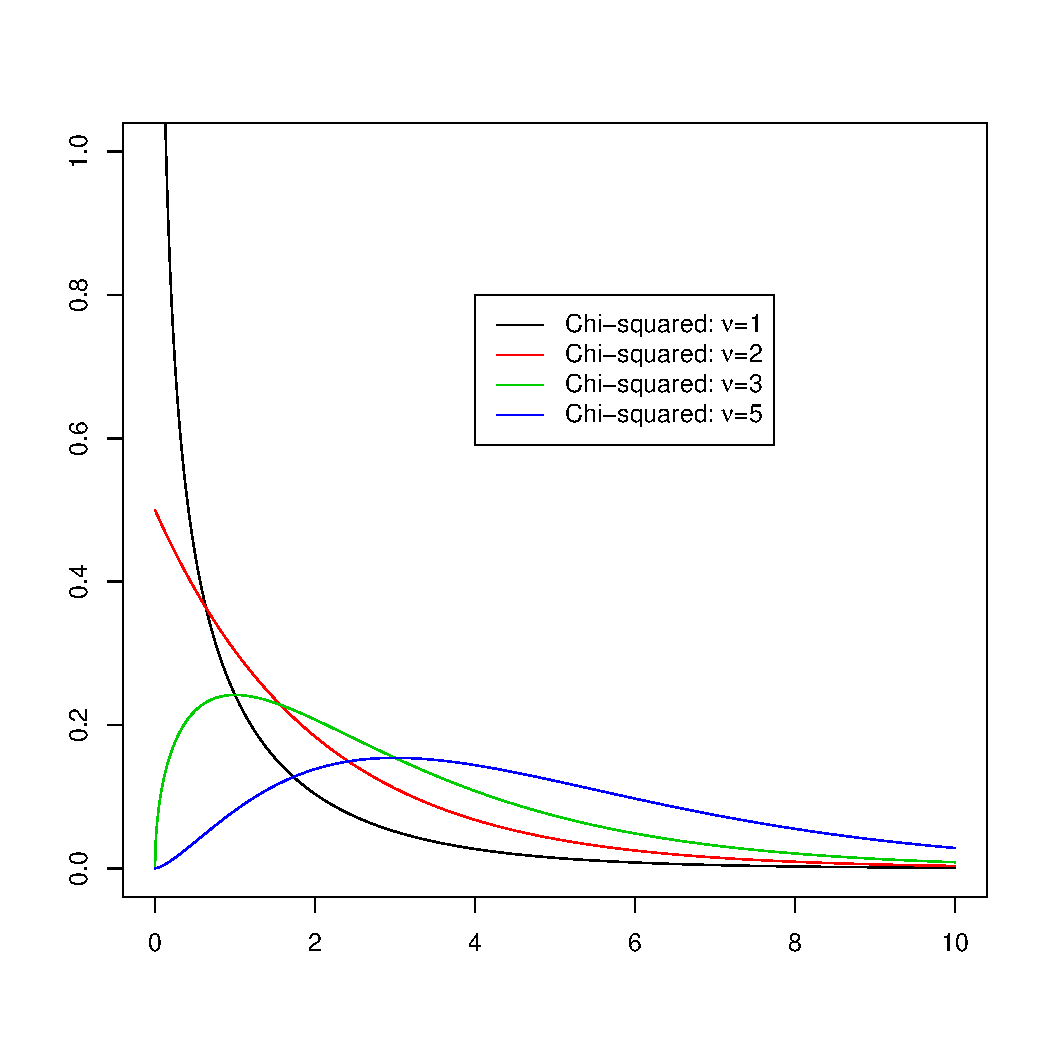
\includegraphics[scale=.5]{chisq.pdf}
\end{center}
\end{frame}

\begin{frame}{Example}
\begin{block}{}
%An article reports the following data on the breakdown voltage of electrically stressed circuits, assumed to be normally distributed:
Recall the breakdown voltage data,  assumed to be normal:
\begin{align*}
&1470, 1510, 1690, 1740, 1900, 2000, 2030, 2100, 2200, \\
& 2290, 2380, 2390, 2480, 2500, 2580, 2190, 2700
\end{align*}
Find a 95\% confidence interval for the standard deviation $\sigma$.
\end{block}

\pause The observed sample mean and sample variance are $\overline X=2126.5$ and $S^2=137324.3$. \pause The critical values are $\chi^2_{.025,16}=28.845$ and $\chi^2_{.975,16}=6.908$, \pause which gives a 95\% confidence interval of
$$\left[\frac{(n-1)S^2}{\chi^2_{\alpha/2,n-1}}, \frac{(n-1)S^2}{\chi^2_{1-\alpha/2,n-1}}\right]
= [76172.3, 318064.4]$$
for $\sigma^2$. \pause The corresponding confidence interval for $\sigma$ is
$$[\sqrt{76172.3}, \sqrt{318064.4}] = [276.0, 564.0]$$
% With
%2
%df 5 n 2 1 5 16, a 95% CI requires x2
%.975,16 5 6.908 and x .025,16 5 28.845. The
%interval is
%a
%16(137,324.3) 16(137,324.3)
%,
%b 5 (76,172.3, 318, 064.4)
%28.845
%6.908
%Taking the square root of each endpoint yields (276.0, 564.0) as the 95% CI for s.

\end{frame}


\begin{frame}{Estimating a Proportion}
Suppose we have a sequence of $n$ Bernoulli trials, where the probability $p$ of success is unknown. If we observe $X$ successes, we know that the maximum likelihood estimator of $p$ is the sample proportion $\hat p=X/n$. 

\vspace{.2cm}\pause How do we construct a confidence interval for $p$ based on $\hat p$?
\pause \begin{block}{}Suppose $X$ is a binomial random variable counting the number of successes in $n$ trials where each trial has probability $p$ of success. If $n$ is sufficiently large an approximate $100(1-\alpha)\%$ confidence interval is given by
$$\hat p \pm z_{\alpha/2}\sqrt{\frac{\hat p(1-\hat p)}n}$$
where $\hat p=X/n$ is the sample proportion, and $z_{\alpha/2}$ is a critical value from the standard normal distribution.
\end{block}
\pause Rule of thumb: This may be used if the number of successes $X$ and the number of failures $n-X$ are both at least 10.
%The sample proportion $\hat p$ has mean $p$ and variance
%$$V(\hat p) = V\left(\frac X n\right) = \frac1{n^2}V(X) = \frac1{n^2}\cdot np(1-p) = \frac{p(1-p)}n$$
%\begin{block}{}
%\end{block}
%\begin{align*}
%S^2 &= \frac1{n-1}(\sum_{i=1}^n {X_i^2}-n\overline{X}^2) \\
%&= \frac1{n-1}(n\hat p-n\hat p^2)
%\end{align*}
\end{frame}

\begin{frame}{Example}
\begin{block}{}
A quality control team for a manufacturer tests 200 randomly selected devices, out of which 15 are defective. Assume that defective devices occur independently of one another. Find an approximate 95\% confidence interval for the proportion defective.
\end{block}
\pause Here the sample proportion is $\hat p=15/200=.075$, and the critical value is $z_{.025}=1.96$, so the approximate 95\% confidence interval is
\begin{align*}
\hat p \pm z_{\alpha/2}\sqrt{\frac{\hat p(1-\hat p)}n} &= .075 \pm 1.96\sqrt{\frac{.075(1-.075)}{200}} \\
&= .075 \pm .037
\end{align*}
\end{frame}

\begin{frame}{Necessary Sample Size for Estimating Proportion}
\begin{block}{}
In the previous example, a $95\%$ confidence interval for the proportion was $.075 \pm .037$. Estimate the required sample size to achieve a margin of error of .01.
\end{block}
\pause Setting the margin of error equal to .01 gives an equation
$$.01=z_{\alpha/2}\sqrt{\frac{\hat p(1-\hat p)}n}$$
\pause Solving for $n$ gives
$$n=\frac{z_{\alpha/2}^2\hat p(1-\hat p)}{.01^2}$$
\pause Unfortunately, this depends on $\hat p$, which is unknown until \textit{after} the new sample is taken. \pause However, we can estimate the required $n$ by using our previous sample proportion $\hat p = .075$:
\pause
$$n \approx \frac{1.96^2(.075)(1-.075)}{.01^2}=2665.11 \approx 2666$$
\end{frame}




\begin{frame}{Summary}
\begin{center}
\small
\renewcommand*{\arraystretch}{1.5}
\begin{tabular}{p{4.5cm}|p{4cm}}
Confidence interval for mean $\mu$ of normal, $\sigma$ known & 
\vspace{-.25cm}$\displaystyle\overline X \pm \frac{z_{\alpha/2}\cdot\sigma}{\sqrt n}$ \\ \hline
Large-sample approximate confidence interval for mean $\mu$ & 
\vspace{-.25cm}$\displaystyle\overline{X} \pm \frac{z_{\alpha/2}\cdot S}{\sqrt{n}}$ \\ \hline
Confidence interval for mean $\mu$ of normal, $\sigma$ unknown & \vspace{-.25cm}$\displaystyle\overline{X} \pm \frac{t_{\alpha/2,n-1}\cdot S}{\sqrt{n}}$ \\ \hline
Prediction interval for normal observation & 
\vspace{-.25cm}$\displaystyle\overline X \pm t_{\alpha/2,n-1}\cdot S\sqrt{1+\frac1n}$ \\ \hline
Confidence interval for variance $\sigma^2$ of normal &
\vspace{-.35cm}$\displaystyle\left[\frac{(n-1)S^2}{\chi^2_{\alpha/2,n-1}}, \frac{(n-1)S^2}{\chi^2_{1-\alpha/2,n-1}}\right]$ \\ \hline
%Confidence interval for mean $\mu$ of exponential & 
%\vspace{-.35cm}$\displaystyle\left[\frac{2\sum_{i=1}^n X_i}{\chi^2_{\alpha/2,2n}} ,\frac{2\sum_{i=1}^n X_i}{\chi^2_{1-\alpha/2,2n}}\right]$ \\ \hline
Approximate confidence interval for proportion $p$ &
\vspace{-.3cm}$\displaystyle\hat p \pm z_{\alpha/2}\sqrt{\frac{\hat p(1-\hat p)}n}$
\end{tabular}
\end{center}
\end{frame}

%% normal sample, conf int for mu, t distribution
%

% prediction interval

%% normal sample, conf int for sigma, chi-squared distribution

\end{document}